Entity selection's primary objective is to reduce the imbalance of a given
entity dimension.
While selecting mesh elements for migration it is important to maintain
inter-part boundaries with low surface area as an increase in the number of
mesh entities classified on boundaries increases application
communications, and in some cases, also the computational
load~\cite{janWhi99}.
Thus, entity selection's secondary objective is to reduce the number of mesh
entities classified on partition model entities of dimension $d<d_{max}$.

Entity selection satisfies the objectives with part-level and entity-level
heuristics.
In Section~\ref{sec:partlvl} we describe how the part-level heuristic
defines a vertex traversal order for evaluating the entity-level
heuristic.
Next, in Section~\ref{sec:entlvl}, we describe how the entity-level heuristic
evaluates the topology of the elements bound by a vertex, a cavity.
Combined, these two procedures reduce both the surface-to-volume ratio of the
parts and their entity imbalance.

\subsection{Part-level Graph Distance Heuristic}\label{sec:partlvl}
The number of mesh entities classified on partition model entities is reduced by
migrating elements from heavily loaded parts that are furthest from the
topological center of the part.
To find these elements we traverse the part boundary vertices in order of their
graph distance.
We define the graph distance of a vertex as the shortest edge-based path between
itself and the part's topological center.
Thus, as diffusive iterations are executed, elements bounding vertices far from
the part's center are migrated and the maximum graph distance of the part
reduced~\cite{diekmann2000shape,meyerhenke2005balancing}.
This approach satisfies the second entity selection objective by forming parts
with lower surface to volume ratios and reduced communications.

To understand the distance computation procedures, we must first account for
parts produced by the graph and geometric partitioning that have multiple
connected components.
We define a (connected) component of a part as the set of elements in which there
exists a path via $M^{d-1}$ adjacencies (faces in 3D) between any two elements.
Given this complexity, we first identify the components, compute the
distance in each component, and then offset the component distances to ensure a
strictly increasing ordering for the boundary traversal; we want the traversal to
process the entire boundary of one component before moving on to the next one.
The remainder of this subsection defines these procedures.

Connected components are identified via a breadth-first $M^{d-1}$
adjacency-based traversal starting at the first mesh element in
the part (based on iterator ordering).
As elements are visited, they are marked with the component id.
When there are no more unmarked $M^{d-1}$ adjacent elements to visit, the
component id is incremented and the traversal is restarted with an unmarked
element in another component.
This process is repeated until all elements in the part are marked with a
component id.

By traversing $M^{d-1}$ mesh adjacencies between elements we have identified
components with the strongest topological connectivity.
But, to compute the graph distance at mesh vertices, we first need to uniquely
assign vertices to components.
For vertices bounded by elements with the same component id the assignment is
obvious.
The problem comes with vertices at the common boundaries between components
formed by lower dimension topological mesh adjacencies (i.e., an edge or vertex
adjacency).
To resolve the assignment issue, we set the vertex id to the lowest bounding
component id.
Now that vertices have vertex component ids, we can find the vertices at the
topological center of each component.

We find the central vertices in a component via a frontal breadth-first traversal.
To begin, we set \texttt{depth} to one and initialize a list \texttt{current}
with all the boundary vertices of a component.
Vertices are then removed from \texttt{current} one-by-one, marked with
\texttt{depth}, and their un-marked edge-adjacent vertices with the same
component id added to a \texttt{next} list.
The lists are then swapped, \texttt{depth} incremented, and the process
repeats.
When there are no more vertices to visit, \texttt{next} is empty, the traversal
ends.
From the set of vertices with the largest \texttt{depth}, the first (based on
vertex iterator ordering) is chosen as the component's central vertex.
The left half of Fig.~\ref{fig:compDistance} shows
the vertices marked with their \texttt{depth}.
From the central vertices Dijkstra's algorithm~\cite{cormen2001introduction} is
run to compute the graph distance to all other vertices in the component.
The topological distance at each vertex is shown in the right half of
Fig.~\ref{fig:compDistance}.
A more complex example of distancing is shown in
Fig.~\ref{fig:oceanTopoDist}.

\begin{figure} [H] \centering
  \includegraphics[width=.42\textwidth]{figs/compDist/2dTreeDepth.png}
  \includegraphics[width=.42\textwidth]{figs/compDist/2dDistance.png}
  \caption{
    (left) The distance from each vertex to the boundary and (right) the
    topological distance from the core vertex (marked with a zero near the
    bottom left corner).
  }
  \label{fig:compDistance}
\end{figure}

%http://texblog.org/2007/08/28/placing-figurestables-side-by-side-subfigure/
\begin{figure} [H] \centering
  \begin{subfigure}{\textwidth}
    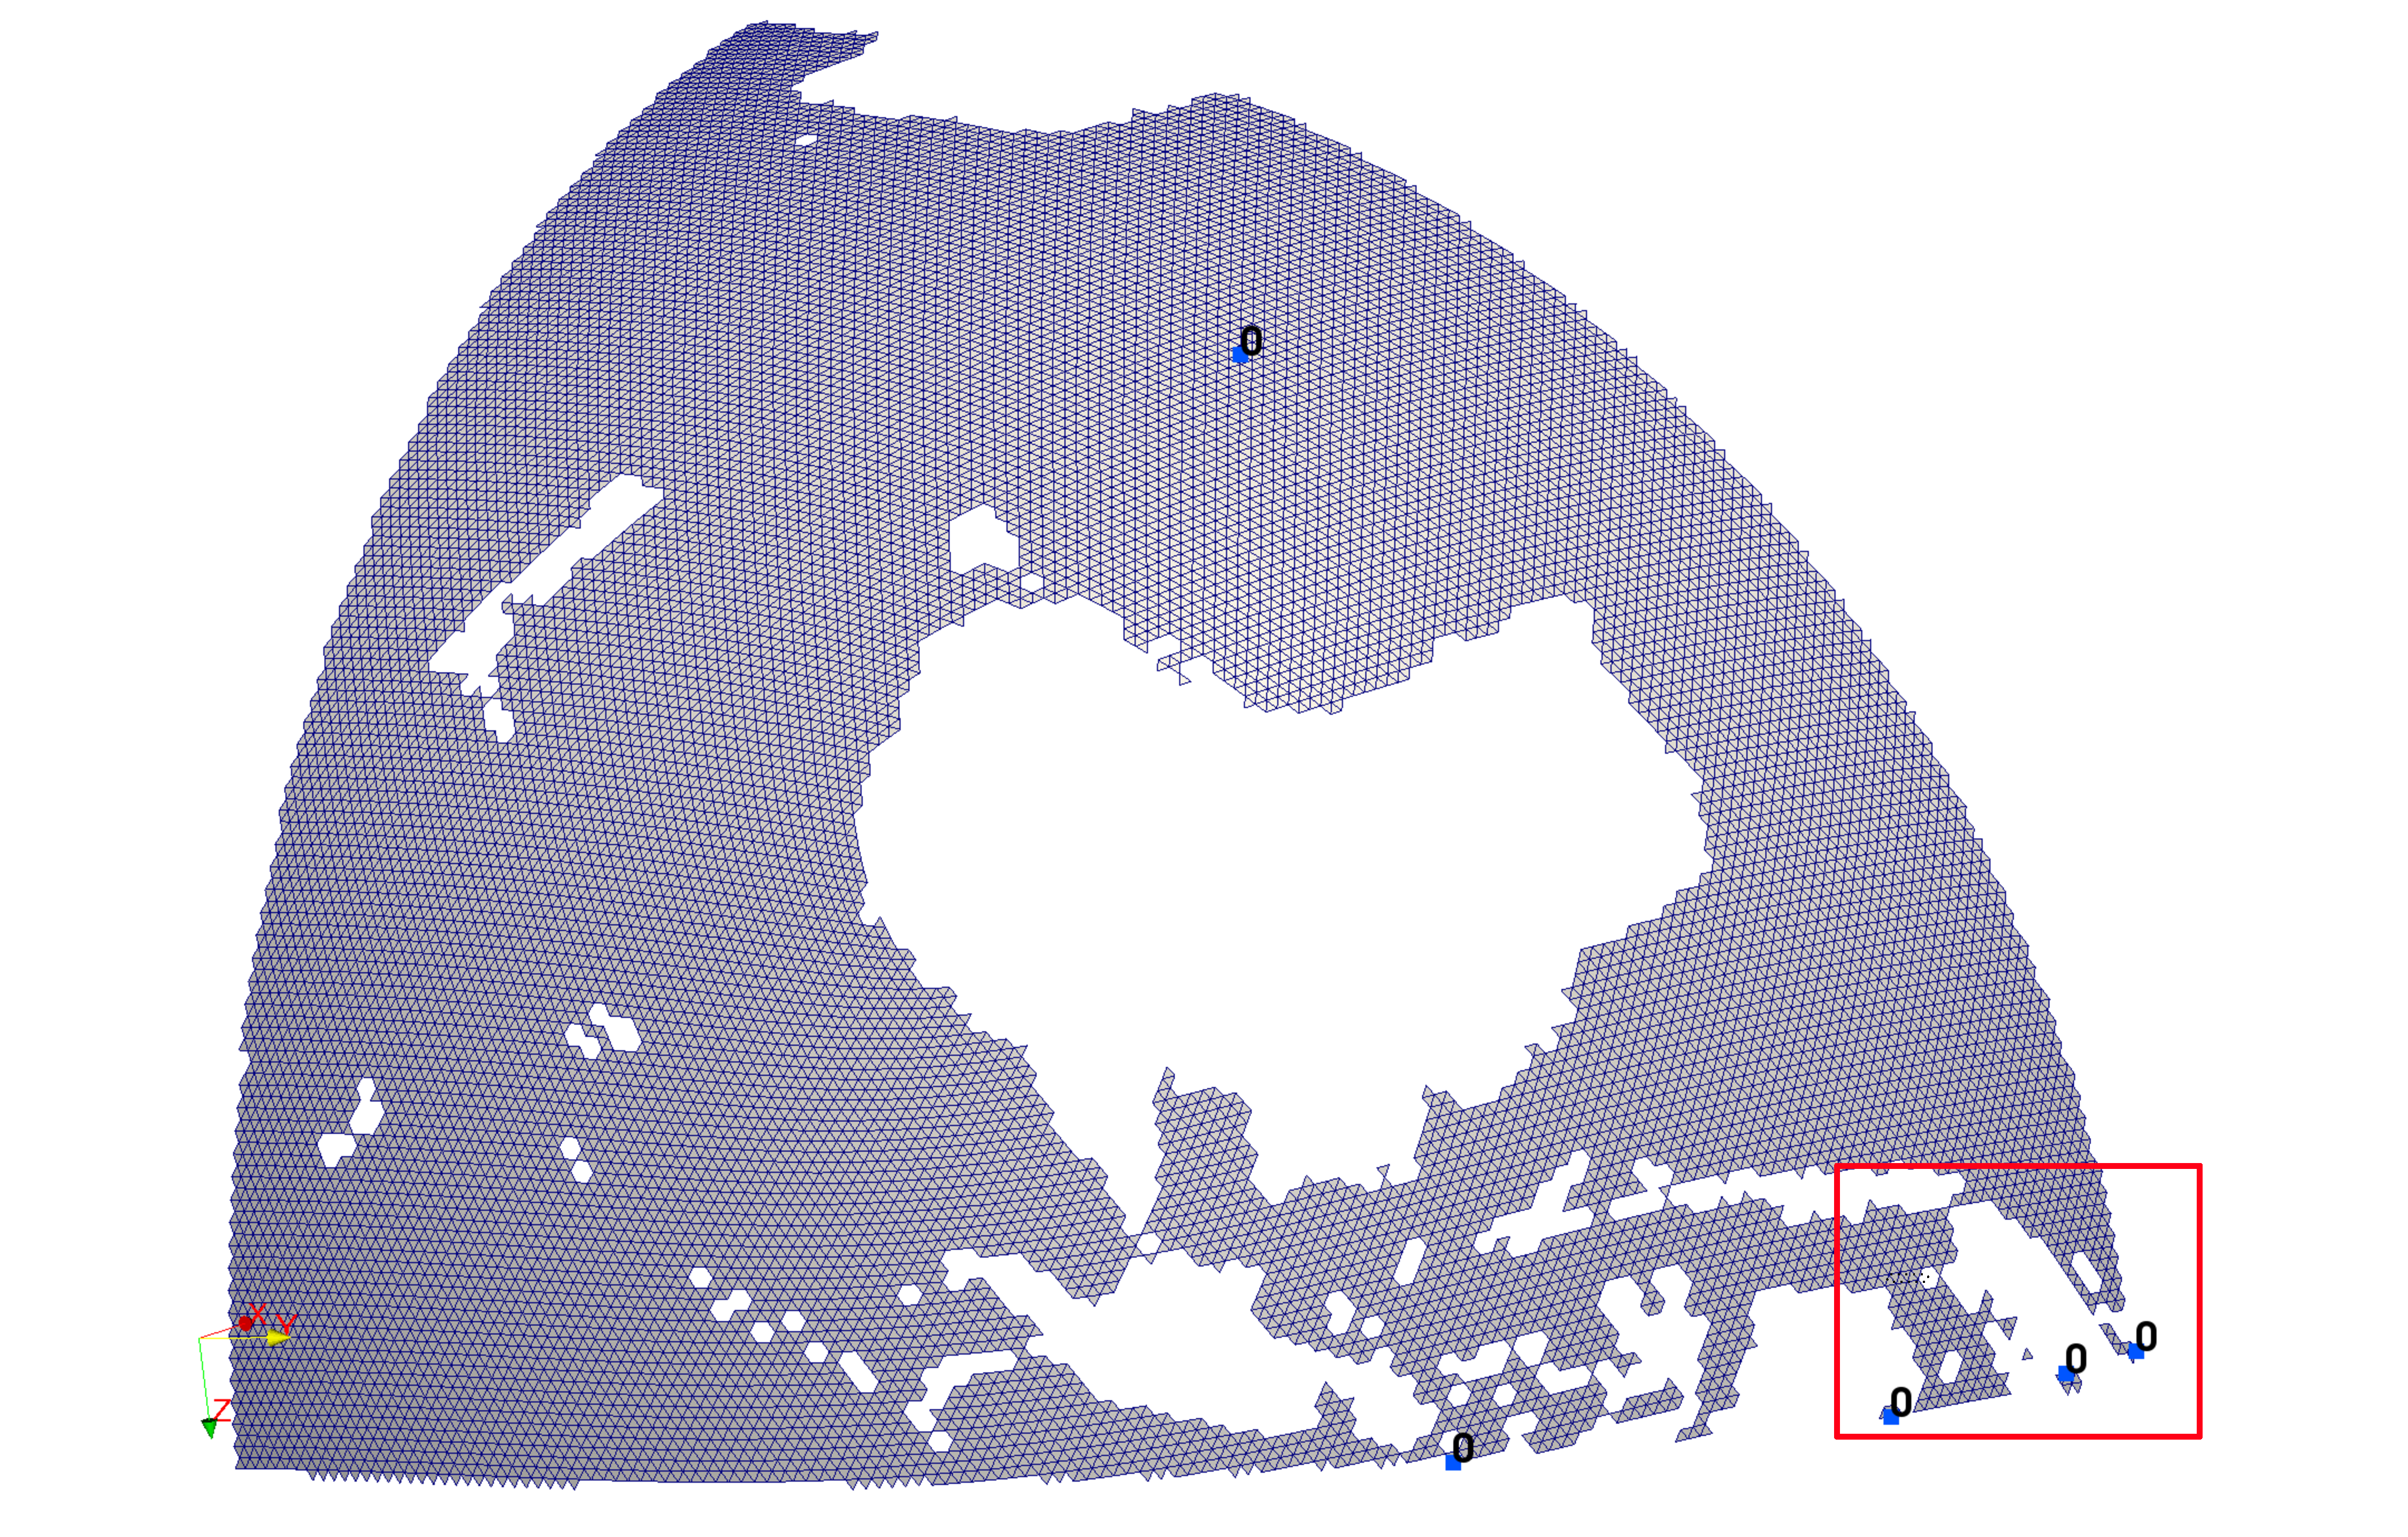
\includegraphics[width=\textwidth]{figs/compDist/p2core.eps}
    \caption{Component core vertices marked with a zero.}
    \label{fig:oceanComps}
  \end{subfigure}
  \begin{subfigure}{.8\textwidth}
    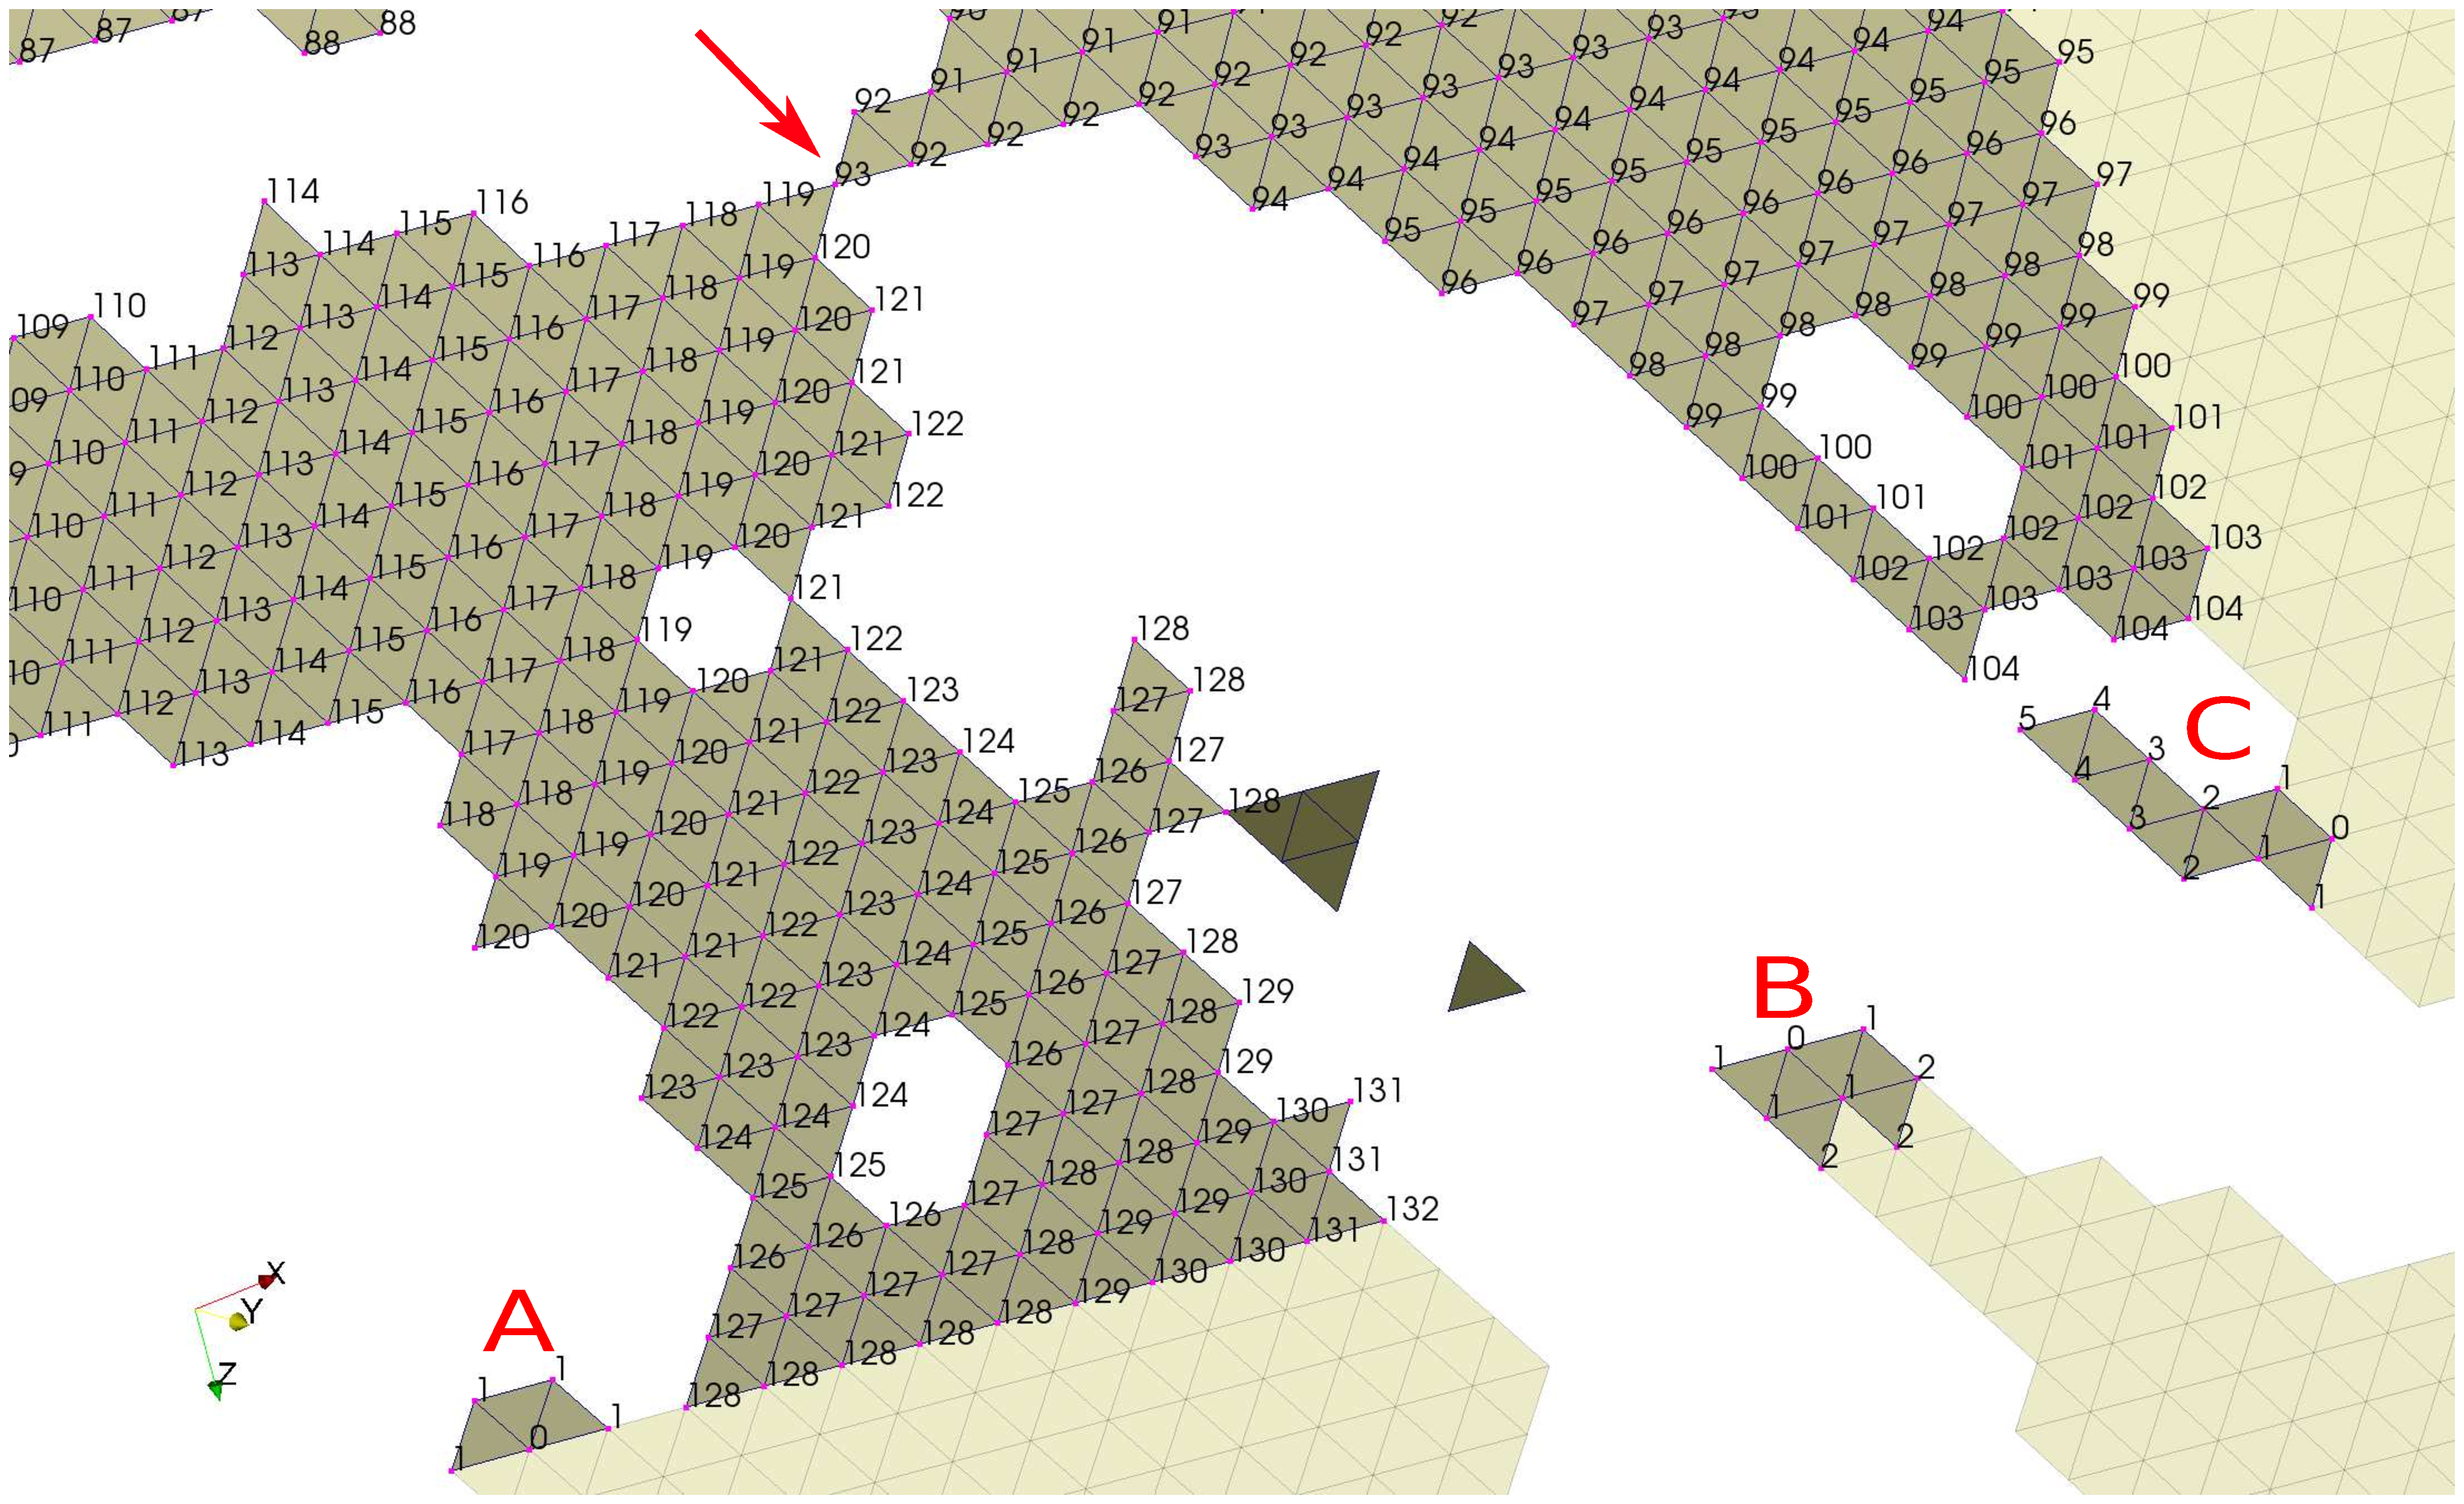
\includegraphics[width=\textwidth]{figs/compDist/p2distComps_nocolor.eps}
    \caption{
      An edge-disconnected junction (arrow) and three disconnected components
      (A, B, C).
    }
    \label{fig:oceanDist}
  \end{subfigure}
  \caption[Components in one of four parts of the MPAS 60km ocean mesh.] {
    Components in one of four parts of the MPAS 60km~\cite{climateMesh} ocean
    mesh.
    Dark shaded elements are isolated (no $M^{d-1}$ adjacency path to elements
    on the part boundary) and light shaded elements are on a different part.
  }
  \label{fig:oceanTopoDist}
\end{figure}

Now that all components have vertices with distance, we must offset the
distances so that our element selection procedure can traverse all the
boundary vertices of a component before moving to another component.
Fig.~\ref{fig:oceanOffset} depicts the distance of
the disconnected components before and after the offset is applied.
Algorithm~\ref{alg:distOff} computes the component vertex
distance, $R(M^0_j)$, offsets.
The procedure begins by sorting the components in order of descending depth;
forming the list $c$.
Next, on Line two, the deepest component, $r_0$, has its offset set to zero.
Lines three through five then compute the offset of the $i^{th}$ component,
$r_i$, by summing the previous component's offset and maximum distance, $r_{i-1} + max(R(M^0_j
\in c(i-1)))$, plus an upper bound on a component's distance increase,
$maxDistIncrease$.
This upper bound enables fast distance updates by including a buffer into the
offset that allows the parts to grow during diffusion iterations without
overlapping.
As each diffusion iteration can only add one layer of elements to a
component, the maximum growth in distance for a component is bounded by
the number of iterations.
So, $maxDistIncrease$ is set to the maximum number of diffusive iterations.
The final step on Line nine loops over the components in ascending order of
their depth and applies the offset to their vertices.
This component traversal order, combined with the conditional checking that the
current distance value is less than the offset, prevents the distance of
vertices on the boundary of two components being offset multiple times.

\begin{figure} [t] \centering
  \includegraphics[width=.25\textwidth]{figs/compDist/p2distComps_nocolor_dccompsA.eps}
  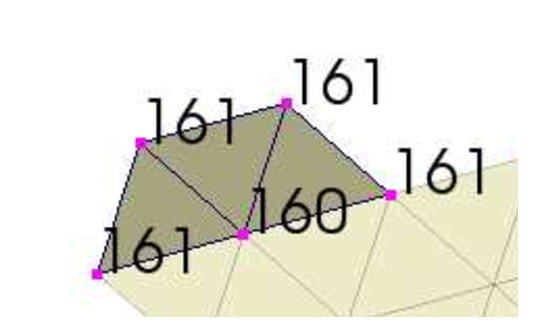
\includegraphics[width=.25\textwidth]{figs/compDist/p2distCompsOff_nocolor_dccompsA.eps}\\
  \includegraphics[width=.25\textwidth]{figs/compDist/p2distComps_nocolor_dccompsB.eps}
  \includegraphics[width=.25\textwidth]{figs/compDist/p2distCompsOff_nocolor_dccompsB.eps}\\
  \includegraphics[width=.25\textwidth]{figs/compDist/p2distComps_nocolor_dccompsC.eps}
  \includegraphics[width=.25\textwidth]{figs/compDist/p2distCompsOff_nocolor_dccompsC.eps}
  \caption[Graph distance of components in the MPAS 60km ocean mesh.]{
    Graph distance of disconnected components A, B, and C from
    Fig.~\ref{fig:oceanTopoDist} (left) before, and (right) after, the offset is
    applied.}
  \label{fig:oceanOffset}
\end{figure}

\begin{algorithm}
  \begin{algorithmic}[1]
  \State c $\leftarrow$ sortDescending(components)
  \State $r_0 \leftarrow 0$   //component zero's offset
  \For{$i \leftarrow 1$, $numComponents$}
     \State $r_i \leftarrow r_{i-1} + max(R(M^0_j \in c(i-1))) + 1 + maxDistIncrease$
  \EndFor
  \For{$i \leftarrow numComponents$, $1$}
    \For{$M^0_j \in c(i)$}
      \If {$R(M^0_j) < r_i$}
        \State $R(M^0_j) \leftarrow R(M^0_j) + r_i$;
      \EndIf
    \EndFor
  \EndFor
  \caption{Vertex Distance Offset}
  \label{alg:distOff}
  \end{algorithmic}
\end{algorithm}

Within a component, detection of non-manifold~\cite{weiler1988radial}
portions of the boundary is critical to ensure that the graph distance
accurately records the shortest $M^{d-1}$ adjacent path from the core to each
vertex.
For example, consider the 2D non-manifold vertex junction
indicated by the arrow in Fig.~\ref{fig:oceanTopoDist}\subref{fig:oceanDist}.
Here the paths from the core vertex marked in the upper portion of
Fig.~\ref{fig:oceanTopoDist}\subref{fig:oceanComps} to either side of the
junction will have significantly different lengths due to the large holes in the
mesh formed by land masses.
Detection of a non-manifold junction at a given boundary vertex, $s$, is through
the breadth-first traversal of $s$'s cavity vertices (i.e., the vertices bounding 
elements in the cavity), rooted at the distance-1 parent of $s$.
Vertices in the cavity are reachable via $M^{d-1}$ adjacencies if the traversal
can visit them without passing through $s$.
For example, consider vertex $s$ in the cavity depicted in Fig.~\ref{fig:cavityPaths} to
have the lowest distance in the priority queue of vertices being processed by
Dijkstra's algorithm.
The detection traversal starts at vertex $p$, the parent of $s$, by enqueuing
vertices $f$ and $h$.
$s$ is also edge-adjacent to $p$, by definition, but it is skipped as paths
through it are not considered.
The traversal continues by dequeuing a vertex and enqueuing its edge-adjacent
vertices that have not been previously visited and are not $s$.
Fig.~\ref{fig:cavityPaths} depicts the depth of each edge in the traversal
tree with hash marks.
If there existed another element that was bounded by $s$ that was also bounded
by $e$ and $d$, or $h$ and $b$, then the edge $(e,d)$ or $(h,b)$ would provide an
edge-adjacent path from $p$ to $b$, $c$ and $d$ and the junction would be
identified as manifold.

\begin{figure} \centering
  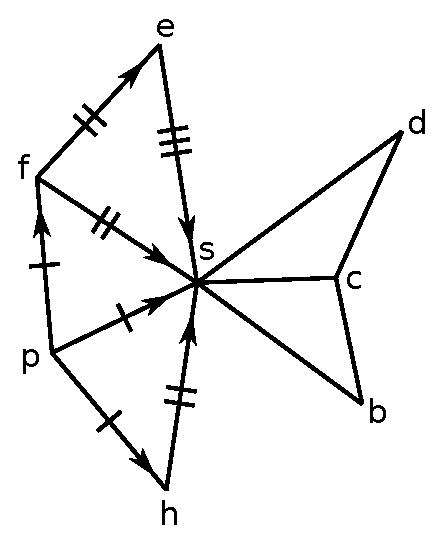
\includegraphics[width=.35\textwidth]{figs/compDist/cavityPaths.eps}
  \caption[Detecting non-manifold component boundaries.]{
    Determining if $s$ is a non-manifold component boundary by creating a cavity
    of elements bounded by $s$, and then trying to walk from its parent vertex
    $p$ to $b$, $c$, or $d$ without going through $s$.
    The hash marks indicate the depth of each edge visited in the walk.
  }
  \label{fig:cavityPaths}
\end{figure}

Compared to LIIPBMod, our part-level heuristic supports improvement of lower
quality partitions by directly accounting for connected components, and
non-manifold junctions within components.

In LIIPBMod, the boundary vertices are iterated over based on the order they
appear in the underlying data structure without consideration for the part
topology.

\subsection{Entity-level Cavity Heuristics}\label{sec:entlvl}
In the previous subsection we described how the part-level heuristic defines a
vertex traversal order for evaluating entity-level heuristics.
In this subsection, we define those entity-level heuristics and how they select
elements for migration to reduce the entity imbalance.
We start by describing size-based cavity selection.
Next, we describe and demonstrate how multiple boundary traversals with
increasing cavity size limits benefit partition improvement.
Lastly, we detail cancellation; a critical mechanism for multi-criteria load
balancing.

Our entity-level, gain-like heuristic~\cite{Fiduccia1982,Kernighan1970} is based
on Zhou's cavity-based approach~\cite{Zhou2010,zhou2012unstructured}, but is
more flexible.
Like LIIPBMod, we check the number of elements in the cavity (the set
of elements adjacent to a vertex on a part boundary), but we also
check the adjacencies within the cavity, and the on- and off-part adjacencies
external to the cavity.
With this additional information we can migrate cavities that are bounded by
vertices classified on partition model vertices, edges, and faces.
\mbox{LIIPBMod's} heuristic avoided multi-part junctions; any cavity whose bounding
vertex is classified on a partition model vertex or edge was not eligible for
migration.
In addition to more flexible migration, our heuristics improve the selection
quality with (1) multiple boundary traversals with increasing cavity size in a
single iteration, (2) allowing migrations to be canceled by the receiver.

The primary check for selection is based on the number of elements in a cavity.
If a cavity is small, then migrating it will decrease the number of entities in
the source part and classified on partition model entities.
Conversely, migrating a face-connected cavity (i.e., between any two elements in
the cavity there exists a path via face adjacencies) with several elements can
result in an increase in the number of mesh entities classified on partition
model entities.
However, migrating small cavities with a few disconnected elements can yield
significant entity reductions.

To illustrate the effect of size and connectivity on entity reductions consider the
cavities depicted in Fig.~\ref{fig:vtxCav} and the reductions listed in
Table~\ref{tbl:entReduction}.
Fig.~\ref{fig:vtxCav} (a-c) and (d-f) respectively depict face-connected and
face-disconnected cavities.
Here, the vertices bounding the cavities are marked with a disc.
Vertices classified on the partition model face $P^2_j$ bounded by parts $P^3_0$
and $P^3_1$ are marked with a circle or disc, and in (c) a vertex classified on a partition
model region, $M^0_i \sqsubset P^3_0$, is marked with a square.
In this example, all elements are migrated from $P^3_0$ to $P^3_1$.
After migration the faces bounded by the circled vertices are now on the part
boundary between $P^3_0$ to $P^3_1$, and in cavities (a-b) and (d-f) there is
one less vertex classified on $P^3_0$.
Migration of cavity (c) does not change the number of entities classified
on the part boundary since there is an entity added to the part boundary
for each one migrated.

%   cavity entities $\sqsubset P^2_j$  
%     a                     b                     c                   
%     before  after delta   before  after delta   before  after  delta
% v   4       3     1       5       4     1       4       4      0    
% e   6       3     3       7       5     2       6       6      0    
% f   3       1     2       4       2     2       3       3      0    
%
%     d                     e                     f                  
%     before  after delta   before  after delta   before  after delta
% v   8       7     1       8       7     1       9       8     1    
% e   15      10    5       16      9     7       17      9     8    
% f   8       4     4       9       3     6       9       3     6    

\begin{figure} [h] \centering
  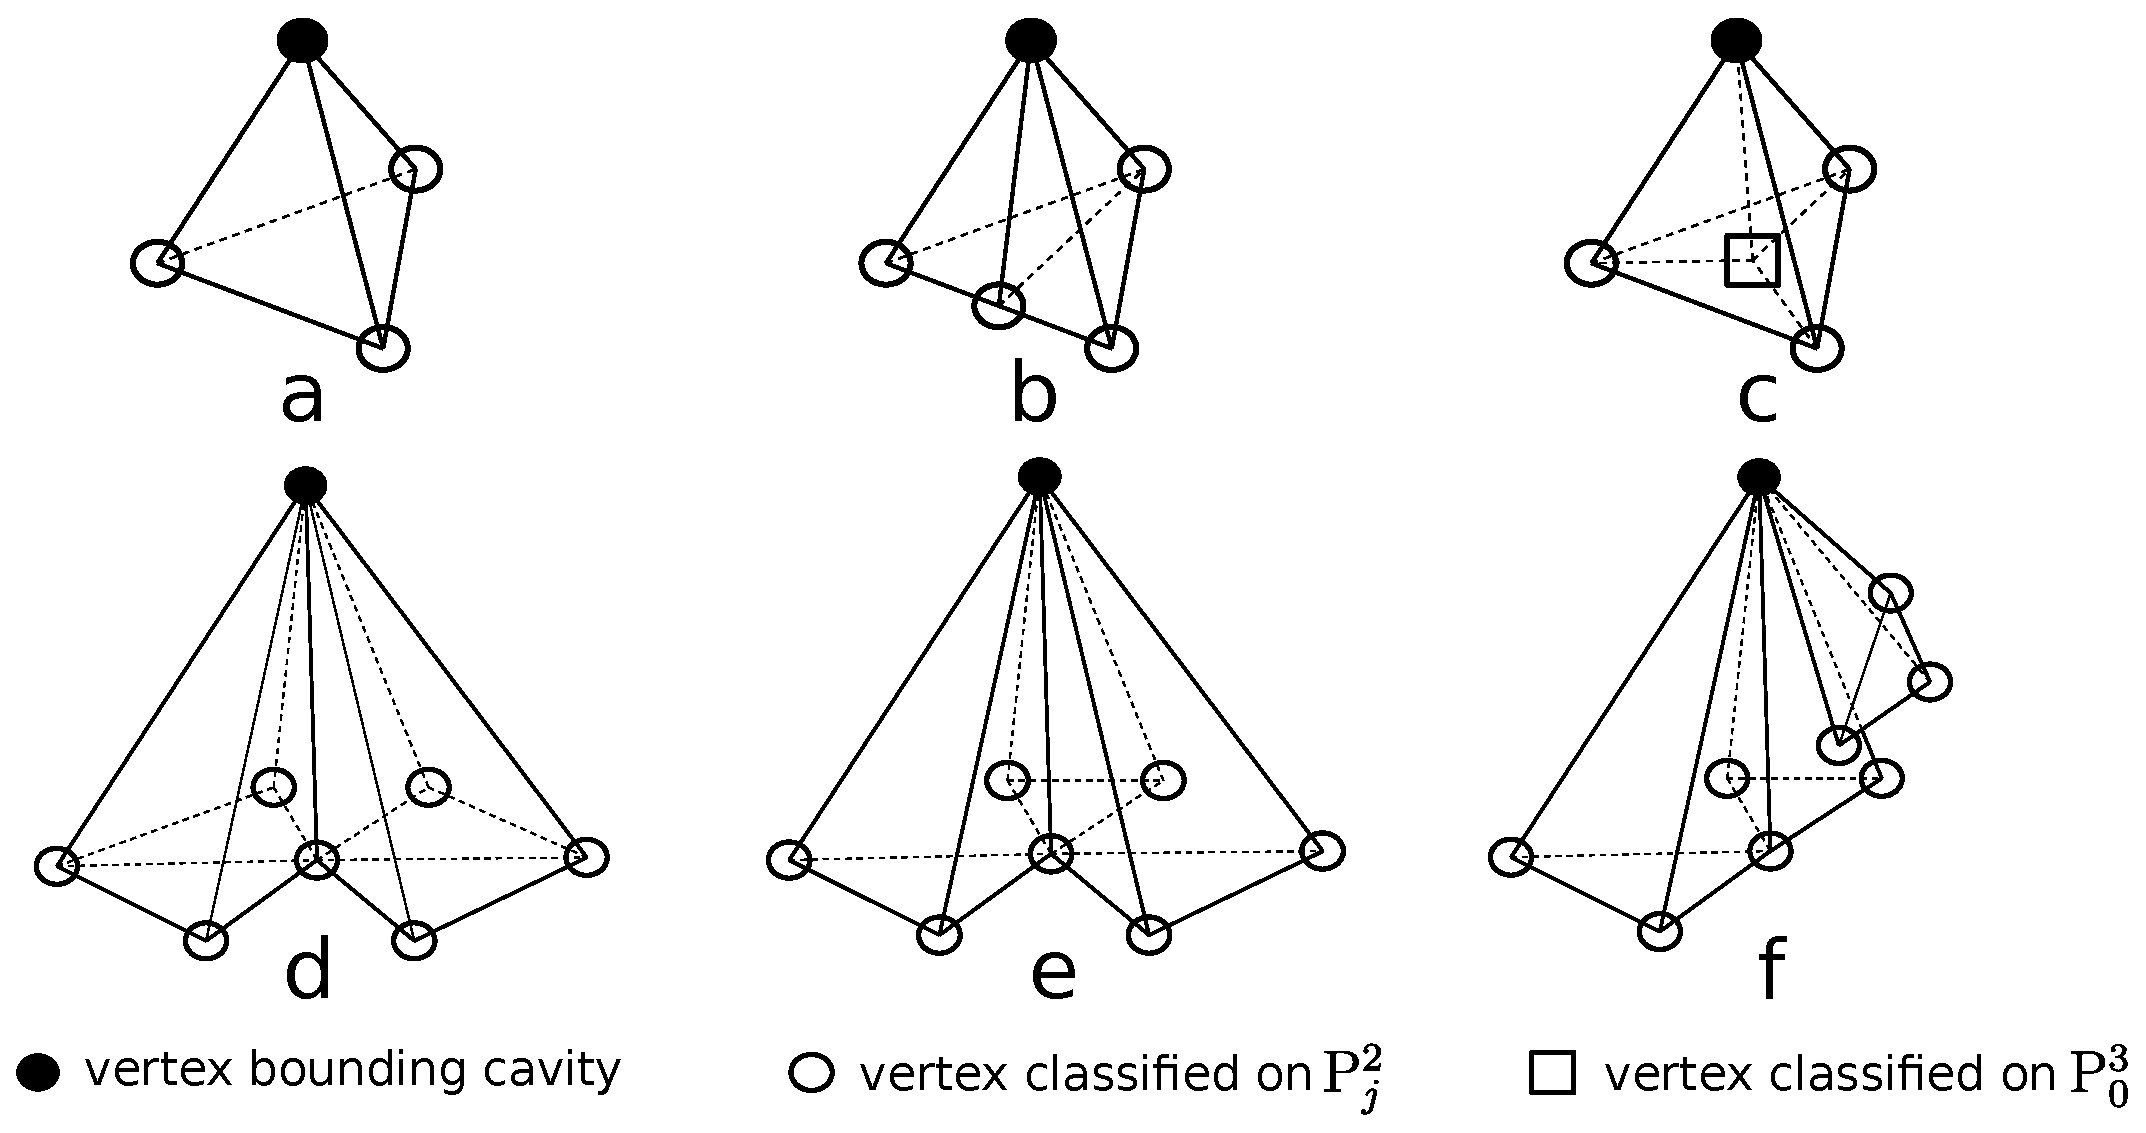
\includegraphics[width=.9\textwidth]{figs/cavities.eps}
  \caption{Vertex bounded cavities being migrated from part 0 to 1.}
  \label{fig:vtxCav}
\end{figure}

\begin{table} [h] \centering
  \footnotesize
  \caption{
    Reduction in the number of mesh entities classified on $P^2_j$ for cavities
    (a-f) depicted in Fig.~\ref{fig:vtxCav}.
  }
  \label{tbl:entReduction}
  \begin{tabular}{l|cccccc}
    & \multicolumn{6}{c}{Cavity} \\
    Entity Dimension & a & b & c & d & e & f \\
    \hline
    Vertex       & 1 & 1 & 0 & 1 & 1 & 1 \\
    Edge         & 3 & 2 & 0 & 5 & 7 & 8 \\
    Face         & 2 & 2 & 0 & 4 & 6 & 6 \\
  \end{tabular}
\end{table}

%DISCUSS multi-pass
Ideally, we would like to select the combination of cavities for migration that
results in the greatest imbalance reductions.
Solving this problem exactly would be expensive, so instead, we iterate over the
part boundary multiple times in order of descending vertex distance while
relaxing (increasing) the cavity size selection limit before executing the PUMI
element migration procedure.
Thus, the first traversal of the boundary will select only cavities with one or
two elements, followed by cavities with less than four elements in the second
traversal (the first traversal may have created new one or two element
candidates), and so on.
The traversal stops at a cavity size limit of 12; roughly half of the average
number of elements adjacent to a vertex in a tetrahedral
mesh~\cite{beall1997general}.

We tested the effectiveness of selection with an increasing size limit
versus a static size limit by balancing a small test mesh.
For both approaches the cavity size limit is set to 12.
The test mesh of the suspension upright has 228 thousand elements and is partitioned to
2048 parts using RIB.
The RIB partition has a perfect element balance and a 53\% vertex imbalance.
Our runs with vertex balancing ParMA targets a 5\% vertex imbalance.
Balancing with the increasing cavity size limit requires 2.0 seconds on 2048
Blue Gene/Q cores.
At the end of the run, the target vertex imbalance is reached, the element
imbalance is 9\%, and the average number of vertices per part is reduced by 3.4\%.
On the same number of cores, the fixed cavity size run takes 3.4 seconds to reach
the target vertex imbalance and has a 15\% element imbalance, and a slight
(0.07\%) increase in the average number of vertices per part.

Once a cavity is selected, it needs to be assigned to a neighboring part for
migration.
The assignment and subsequent migration should result in a reduction of the
number of mesh entities classified on the part boundary.
In a 3D mesh we assign the cavity to the part that shares the most mesh edges
with it.
Counting shared edges avoids counting vertices (the lowest dimension shared entity)
that are not adjacent to a higher dimension shared entity (an edge or a face) while
providing more information than the counting of shared faces (the highest
dimension shared entity, in 3D).
Fig.~\ref{fig:cavityPeers} depicts a two element cavity with entities
classified on both partition model faces and edges.
Specifically, the cavity has two faces shared with part one (dark shaded), two
faces with part two (unshaded),
and an additional classification of edge F on the partition model
edge shared with part two (dashed line in bold).
Counting shared edges correctly identifies part two as the destination;
it has six cavity edges versus part one only having five.
The `Sum' row of Table~\ref{tbl:cavityPeerEnts} lists the total cavity edge
count on each part when the cavity elements are owned by part zero, the initial
owner, and parts one and two, the two possible target parts.
For this example, migrating the cavity to part two reduces the total number of
shared edges from 20 to 19; if part one were selected the total number of shared
edges would increase by one.
If multiple parts are tied for the most shared edges then the first part with
remaining capacity is selected as the destination.

\begin{figure} \centering
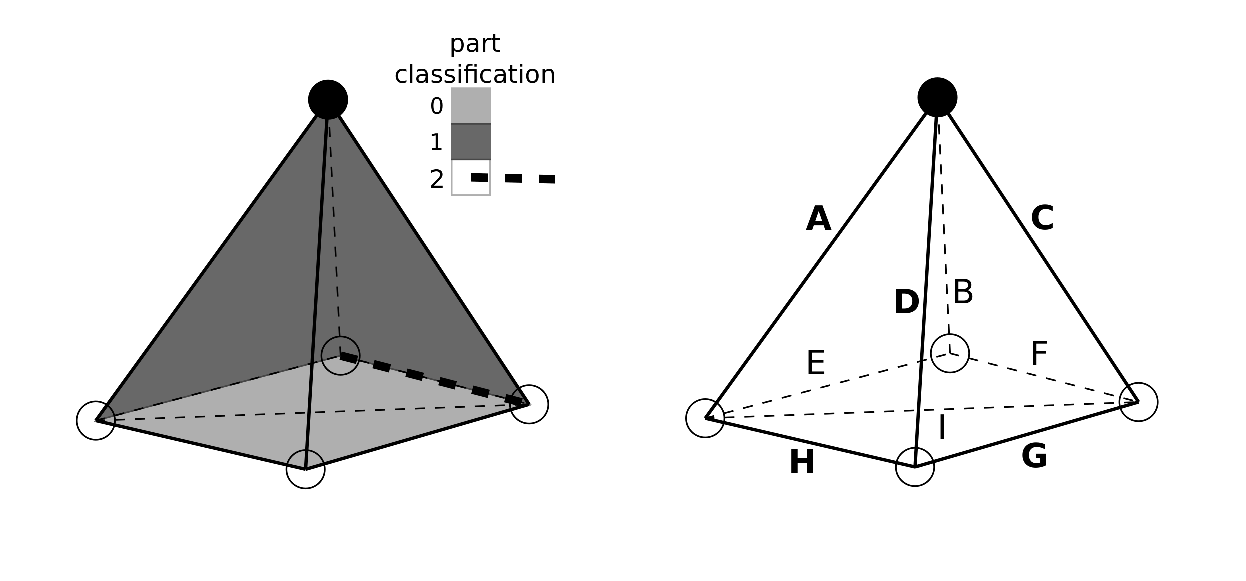
\includegraphics[width=.8\textwidth]{figs/cavityPeers/cavityPeers-shaded.eps}
\caption[Counting mesh entity partition model classification to select a destination
         part for the cavity elements.] {
    Counting mesh entity partition model classification to select either part
    one or part two for the migration of part zero cavity elements.
    The cavity bounding vertex is marked with a disc.
    (left) Part classification; faces in the foreground
    classified on part 2 are not shaded.
    (right) Mesh edge labels. For clarity, edges in the
    foreground have bold labels.
}
\label{fig:cavityPeers}
\end{figure}

\begin{table} \centering
  \footnotesize
  \caption[Existence of Fig.~\ref{fig:cavityPeers} cavity edges on parts.]{
    Existence of Fig.~\ref{fig:cavityPeers} cavity edges on parts.
    The column groups list the edge existence prior to migration of the cavity
    (Owner=0), and after migration to part $N$ (Owner=$N$).
    An entry is `1' if the edge exists on the part.  The last row
    lists the total number of cavity edges on each part.
  }
  \label{tbl:cavityPeerEnts}
  \begin{tabular}{cc|ccc|ccc|ccc}
            & & \multicolumn{9}{c}{Cavity Owner} \\
            &  & \multicolumn{3}{c|}{0}
            & \multicolumn{3}{c|}{1}
            & \multicolumn{3}{c}{2} \\
    \hline
           & Part & 0 & 1 & 2 & 0 & 1 & 2 & 0 & 1 & 2\\
    \hline
           & A    & 1 & 1 & 1 & 0 & 1 & 1 & 0 & 1 & 1 \\
           & B    & 1 & 1 & 0 & 0 & 1 & 0 & 0 & 1 & 1 \\
           & C    & 1 & 1 & 1 & 0 & 1 & 1 & 0 & 1 & 1 \\
           & D    & 1 & 0 & 1 & 0 & 1 & 1 & 0 & 0 & 1 \\
    Edge   & E    & 1 & 1 & 0 & 1 & 1 & 0 & 1 & 1 & 1 \\
           & F    & 1 & 1 & 1 & 1 & 1 & 1 & 1 & 1 & 1 \\
           & G    & 1 & 0 & 1 & 1 & 1 & 1 & 1 & 0 & 1 \\
           & H    & 1 & 0 & 1 & 1 & 1 & 1 & 1 & 0 & 1 \\
           & I    & 1 & 0 & 0 & 1 & 1 & 0 & 1 & 0 & 1 \\
    \hline
           & Sum  & 9 & 5 & 6 & 6 & 9 & 6 & 5 & 5 & 9 \\
  \end{tabular}
\end{table}

%DISCUSS weight tracking
As the part boundary is traversed and the cavity heuristic selects elements for
migration, the weight of the selected entities is tracked to prevent migrating too
much weight to the target parts.
Tracking is based on the simple rule, rooted in the unique assignment of
elements to parts, that an entity will not exist on the part if all the elements
it bounds are marked for migration.
Thus, the weight tracking mechanism checks for this condition, and if satisfied,
adds the entities weight to the running total for the given destination part.

%DISCUSS cancellation
During the balancing of lower priority entity dimensions (e.g., elements during
vertex $>$ element balancing) the imbalance of higher priority entity dimensions is
preserved by canceling the migration of some elements~\cite{schloegel1997multilevel}.
First, the sending parts determine how much weight associated with higher
priority entities is migrated to the target parts.
These weights are then sent to the respective targets using PCU's neighborhood
communication procedures~\cite{ibanez2016hybrid}.
The target part then iterates over the incoming migration requests in descending
order of the migration weight, accepts the request if capacity remains, reduces
the remaining capacity accordingly, and sends the accepted weight to the sender.
The sending part then traverses the list of migration elements in the order they
were selected (i.e., descending distance from the parts topological core), and keeps
elements in the list until the peer's higher priority entity weight capacity is
exceeded.
A summary of the interaction between the part-level and entity-level heuristics
is given in Section~\ref{sec:complexity}.

\subsection{Stagnation Avoidance}\label{sec:stagnation}
A stagnation~\cite{Zhou2010} avoidance procedure stops execution of diffusion
when the imbalance or part shape has not improved over several iterations.
Specifically, a second order accurate backward finite
difference~\cite{fornberg1988generation} approximates the rate of change of the
imbalance, \textit{imb}, and the average number of boundary mesh
vertices per part, \textit{sides}.
Diffusion is stopped if the rate of change in \textit{imb} is less than one
percent of the target imbalance and the change in \textit{sides} is less than
one-hundredth of the initial \textit{sides}.

\subsection{Time Complexity}\label{sec:complexity}

The part-level heuristic requires first executing an $O(|M^d|+|M^{d-1}|)$
element-based, breadth-first traversal to identify disconnected components.
Next, the vertex component ids are set, $O(|M^0|)$, and boundary vertices
are inserted into STL sets, $O(|M^0|log|M^0|)$.
The component vertices are then traversed in breadth-first order via edge
adjacencies to locate the topological center, $O(|M^0|+|M^{1}|)$.
For simplicity, our implementation uses an STL set to maintain the vertices at
each tree-depth.
This choice adds $O(|M^0|log|M^0|)$ to the cost and could be avoided with a
list-based traversal.
Next, Dijkstra's algorithm is run to compute vertex distances,
$O(|M^1|+|M^0|log|M^0|)$.
As the vertices are visited, adjacent elements are accessed for non-manifold
topology detection; a cost increase of $O(|M^d|)$.
Lastly, the vertex distances are offset, $O(|M^0|)$.
The overall complexity of the part-level heuristic for a 3D tetrahedral mesh is
$O(|M^1| + |M^2| + |M^3| + |M^0|log|M^0|)$.
But, for each entity dimension being balanced these procedures only need to be
executed once.
In subsequent iterations we can execute a lower cost distance update on just the
boundary vertices.

In each iteration the entity-level heuristic first requires building a STL
map-based distance queue of vertices to traverse, $O(|M^0|log|M^0|)$.
The vertices in the queue are then traversed, $O(|M^0|)$, and cavities
constructed by adjacent element queries, $O(|M^d|)$.
Lastly, the cavity edges are queried for determining the destination part,
$O(|M^1|)$.
Thus, the entity-level heuristic's complexity is
$O(|M^0|log|M^0| + |M^1| + |M^d|)$.

A detailed analysis of convergence and overall time complexity of general
diffusive load balancing procedures can be found in the work of
Subramanian~\cite{subramanian1994analysis} and Berenbrink~\cite{berenbrink2009}.
